%%%%%%%%%%%%%%%%%%%% author.tex %%%%%%%%%%%%%%%%%%%%%%%%%%%%%%%%%%%
%
% sample root file for your "contribution" to a contributed volume
%
% Use this file as a template for your own input.
%
%%%%%%%%%%%%%%%% Springer %%%%%%%%%%%%%%%%%%%%%%%%%%%%%%%%%%


% RECOMMENDED %%%%%%%%%%%%%%%%%%%%%%%%%%%%%%%%%%%%%%%%%%%%%%%%%%%
\RequirePackage{amsmath}
\documentclass[graybox]{svmult}

% choose options for [] as required from the list
% in the Reference Guide

\usepackage{amssymb}       % selects Times Roman as basic font
\usepackage{helvet}         % selects Helvetica as sans-serif font
\usepackage{courier}        % selects Courier as typewriter font
\usepackage{type1cm}        % activate if the above 3 fonts are
                            % not available on your system
%
\usepackage{makeidx}         % allows index generation
\usepackage{graphicx}        % standard LaTeX graphics tool
                             % when including figure files
\usepackage{multicol}        % used for the two-column index
\usepackage[bottom]{footmisc}% places footnotes at page bottom

\usepackage{psfrag,bbm,epsf}
\usepackage{amssymb, color,enumerate,float,mathtools,algorithmicx}
\usepackage{algorithm}
\usepackage[numbers]{natbib}
\usepackage{enumerate,multirow,booktabs}
\usepackage{url}
\usepackage{natbib}

\newcommand{\blind}{1}
\newtheorem{lem}{Lemma}
\newtheorem{thm}{Theorem}
\newtheorem{pro}{Proposition}
\newtheorem{defn}{Definition}
\newtheorem{rmk}{Remark}
\newtheorem{cor}{Corollary}
\newcommand{\reals}{\mathbb{R}}
\newcommand{\naturals}{\mathbb{R}}
\newcommand{\vc}{\boldsymbol{c}}
\newcommand{\vx}{\boldsymbol{x}}
\newcommand{\vt}{\boldsymbol{t}}
\newcommand{\vz}{\boldsymbol{z}}
\newcommand{\vu}{\boldsymbol{u}}
\newcommand{\vy}{\boldsymbol{y}}
\newcommand{\vinfty}{\boldsymbol{\infty}}
\newcommand{\vzero}{\boldsymbol{0}}
\newcommand{\vPsi}{\boldsymbol{\Psi}}
\newcommand{\dif}{{\rm d}}
\DeclareMathOperator{\sign}{sign}
\newcommand{\Udes}{\mathcal{U}}
\newcommand{\Xdes}{\mathcal{X}}
\newcommand{\FXdes}{F_{\Xdes}}
\newcommand{\cm}{\mathcal{M}}
\newcommand{\Ftar}{F}
\newcommand{\ftar}{\varrho}
\newcommand{\cube}{\ensuremath{(0,1)^d}}
\newcommand{\bbone}{\mathbbm{1}}
\newcommand{\ip}[3][{}]{\ensuremath{\left \langle #2, #3 \right \rangle_{#1}}}
\newcommand{\norm}[2][{}]{\ensuremath{\left \lVert #2 \right \rVert}_{#1}}

\def\abs#1{\ensuremath{\left \lvert #1 \right \rvert}}

\usepackage{bm} %to get bold math fonts

\newcommand{\FJH}[1]{{\color{blue}Fred: #1}}
\newcommand{\LK}[1]{{\color{green}Lulu: #1}} %choose your color
\newcommand{\YL}[1]{{\color{red}Yiou: #1}} %choose your color

% see the list of further useful packages
% in the Reference Guide

\makeindex             % used for the subject index
                       % please use the style svind.ist with
                       % your makeindex program

%%%%%%%%%%%%%%%%%%%%%%%%%%%%%%%%%%%%%%%%%%%%%%%%%%%%%%%%%%%%%%%%%%%%%%%%%%%%%%%%%%%%%%%%%

\begin{document}

\title*{Are Transformed Low Discrepancy Points Also Low Discrepancy?}
% Use \titlerunning{Short Title} for an abbreviated version of
% your contribution title if the original one is too long
\author{Yiou Li, Lulu Kang, and Fred Hickernell}
% Use \authorrunning{Short Title} for an abbreviated version of
% your contribution title if the original one is too long
\institute{Yiou Li \at DePaul University, 1 E. Jackson
Chicago, IL 60604, \email{yli139@depaul.edu}
\and Lulu Kang \at Illinois Institute of Technology, 10 W 32nd Street, Chicago, IL 60616 \email{lkang2@iit.edu} 
\and 
Fred Hickernell \at Illinois Institute of Technology, 10 W 32nd Street, Chicago, IL 60616 \email{hickernell@iit.edu}}
%
% Use the package "url.sty" to avoid
% problems with special characters
% used in your e-mail or web address
%
\maketitle

\abstract{Write me later}

\section{Introduction}

Professor Kai-Tai Fang and his collaborators have demonstrated the effectiveness of low discrepancy points as space filling designs \cite{FanWan94, FanLiSud06, FangHic07a}.  
They promoted discrepancy as a quality measure for statistical experimental designs to the statistics, science, and engineering communities \cite{FanMaWin02, FanMuk00, FanMa01a, FanMa01b}. 

Low discrepancy designs, $\Udes = \{\vu_i\}_{i=1}^N$, are typically constructed so that their empirical distribution, $F_\Udes$, approximates $F_u$, the uniform distribution on the unit cube, \cube.  
The discrepancy measures how large $F_u-F_\Udes$ is.  

When the target distribution for the design, $\Ftar$, defined over the experimental domain $\Omega$, is \emph{not} the uniform distribution on the unit cube, then one typically constructs the desired design, $\Xdes$, by transforming a low discrepancy uniform design, i.e., 
\begin{equation} \label{eq:transPts}
\Xdes = \{\vx_i\}_{i=1}^N = \{\vPsi(\vu_i)\}_{i=1}^N = \vPsi(\Udes), \qquad \vPsi: \cube \to \Omega.
\end{equation}
Note that $\Ftar$ may differ from $F_u$ because $\Omega \ne \cube$ and/or $\Ftar$ is non-uniform.  
A natural transformation, $\vPsi$, when $\Ftar$ has independent marginals is the inverse distribution transformation:
\begin{equation}\label{eq:inverse}
\Psi_j(u_j) = F_j^{-1}(u_j), \quad \text{where } \Ftar(\vx) = F_1(u_1) \cdots F_d(u_d).
\end{equation}
A number of transformation methods for different distributions can be found in \cite{devroye2006nonuniform}. 

The question addressed in this chapter is whether the design $\Xdes$ resulting from transformation \eqref{eq:transPts} of a low discrepancy design, $\Udes$, is itself low discrepancy with respect to the target distribution $\Ftar$. 
In other words, 
\begin{equation} \label{BigQ} \tag{Q}
\text{\emph{does small $F_u - F_\Udes$ imply small $\Ftar - F_\Xdes$?}}
\end{equation}
We demonstrate that the answer may be yes or no, depending on how the question is posed.  
We discuss both cases.  
For illustrative purposes, we consider the case where $\Ftar$ is the multivariate normal distribution.

In the rest of this chapter, we first explain the discrepancy that measures how large $\Ftar - F_\Xdes$ is and motivate it from three different perspectives.  Next, we the inverse transformation can lead to inconsistency in terms the discrepancies of the designs before and after transformation. 
We also proposed a remedy method to improve the design in terms of the discrepancy between $\Ftar$ and $F_\Xdes$. 
Numerical examples are used to show the performance of the method. 

%%%%%%%%%%%%%%%%%%%%%%%%%%%%%%%%%%%%%%%%%%%%%%%%%%%%%%%%%%%%%%%%%%%%%%%
%%%%%%%%%%%%%%%%%%%%%%%%%%%%%%%%%%%%%%%%%%%%%%%%%%%%%%%%%%%%%%%%%%%%%%%
\section{The Discrepancy}
%%%%%%%%%%%%%%%%%%%%%%%%%%%%%%%%%%%%%%%%%%%%%%%%%%%%%%%%%%%%%%%%%%%%%%%
%%%%%%%%%%%%%%%%%%%%%%%%%%%%%%%%%%%%%%%%%%%%%%%%%%%%%%%%%%%%%%%%%%%%%%%

Experimental design theory based on  discrepancy assumes an experimental region, $\Omega$, and a target probability distribution, $\Ftar:\Omega \to [0,1]$, which is known a priori. In many of our examples, we assume that $\Ftar$ has a probability density, $\ftar$.  It is convenient to also work with measures, $\nu$, defined on $\Omega$.  If $\nu$ is a probability measure, the associated probability distribution is given by $F(\vx) = \nu((-\vinfty,\vx])$.  The Dirac measure, $\delta_{\vx}$ is the probability measure assigning unit measure to the point $\vx$.  A design, $\Xdes = \{\vx_i\}_{i=1}^N$, is a finite set of points that has an associated empirical distribution, $F_{\Xdes}  = N^{-1} \sum_{i=1}^N \bbone_{(-\vinfty,\vx_i]}$ as well as an associated empirical measure, $\nu_{\Xdes}  = N^{-1} \sum_{i=1}^N \delta_{\vx_i}$.

In the remainder of this section we provide three interpretations of the discrepancy---the magnitude of $\Ftar - \FXdes$.  One interpretation is the norm of $\Ftar - \FXdes$.  The second interpretation is worst-case cubature error for integrands in a Hilbert space.  The third interpretation is average case cubature error for stochastic processes.

%%%%%%%%%%%%%%%%%%%%%%%%%%%%%%%%%%%%%%%%%%%%%%%%%%%%%%%%%%%%%%%%%%%%%%%
\subsection{Definition in Terms of a Norm on a Hilbert Space of Measures}
%%%%%%%%%%%%%%%%%%%%%%%%%%%%%%%%%%%%%%%%%%%%%%%%%%%%%%%%%%%%%%%%%%%%%%%

Let $(\cm, \ip[\cm]{\cdot}{\cdot})$ be a Hilbert space of measures defined on the experimental region, $\Omega$.  Assume that $\cm$ includes all Dirac measures.  Define the function $K:\Omega \times \Omega \to \reals$ in terms of inner products of Dirac measures:
\begin{equation} \label{kerDeltaDef}
    K(\vt,\vx) := \ip[\cm]{\delta_{\vt}}{\delta_{\vx}}, \qquad \forall \vt, \vx \in \Omega.
\end{equation}
It is straightforward to show that $ K$ is symmetric in its arguments and positive-definite, namely:
\begin{gather*}
K(\vx, \vt) = K(\vt, \vx) \qquad \forall \vt, \vx\in \Omega,\\
\sum\limits_{i, k=1}^N c_i c_k  K(\vx_i,\vx_k) > 0, \qquad \forall N\in\mathbb{N}, \  \vc \in\mathbb{R}^N, \ \vc \ne \vzero,  \ \Xdes \in\Omega.
\end{gather*}
For arbitrary measures $\lambda, \nu \in \cm$, their inner product can be expressed in terms of a double integral of the kernel, $K$:
\begin{equation} \label{ipMdef}
    \ip[\cm]{\lambda}{\nu} = \int_{\Omega \times \Omega} K(\vt,\vx) \, \lambda(\dif \vt) \nu(\dif \vx).
\end{equation}
This can be established directly from \eqref{kerDeltaDef} for $\cm_0$, the vector space spanned by all Dirac measures.  Letting $\cm$ be the closure of the pre-Hilbert space $\cm_0$ then yields \eqref{ipMdef}.

The discrepancy of the design $\Xdes$ with respect to the target probability measure $\nu$ using the kernel $K$, can be defined as the norm of the difference between the target probability measure, $\nu$, and the empirical probability measure for $\Xdes$:
\begin{subequations} \label{discDef}
\begin{align} 
    D^2(\Xdes,\nu,K) & := \norm[\cm]{\nu - \nu_{\Xdes}}^2 = \int_{\Omega \times \Omega} K(\vt,\vx) \, (\nu - \nu_{\Xdes})(\dif \vt) (\nu - \nu_{\Xdes})(\dif \vx) \\
    \nonumber
    & = \int_{\Omega \times \Omega} K(\vt,\vx) \, \nu(\dif \vt) \nu (\dif \vx)\\
    & \qquad \qquad - \frac 2N \sum_{i=1}^N \int_{\Omega} K(\vt,\vx_i) \, \nu(\dif \vt) + \sum_{i,k=1}^N K(\vx_i,\vx_k).
\end{align}
The first argument refers to the design, the second to the target measure, and the third refers to the kernel used to define the kernel used to define the Hilbert space norm for $\cm$.
The formula for the discrepancy may be written equivalently in terms of the probability density, $\rho$, corresponding to the probability measure, $\varrho$:
\begin{align}
\nonumber
    D^2(\Xdes,\varrho,K)  & = \int_{\Omega \times \Omega} K(\vt,\vx) \, \varrho(\vt) \varrho (\vx) \, \dif \vt\dif \vx\\
    & \qquad \qquad - \frac 2N \sum_{i=1}^N \int_{\Omega} K(\vt,\vx_i)  \, \varrho(\vt) \, \dif \vt + \sum_{i,k=1}^N K(\vx_i,\vx_k).
\end{align}
\end{subequations}
Here, and below we abuse the notation for discrepancy, but we always preserve the meaning of the first second and third arguments.  Thus,
\[
D(\Xdes,\nu,K), \ D(\Xdes,F,K), \ D(\Xdes,\varrho,K), \ D(\nu_{\Xdes},\nu,K), \text{ etc.} 
\]
are all equivalent.

The equivalent formulas for the discrepancy in \eqref{discDef} depend inherently on the choice of $K$.  That is key to the answering our question \eqref{BigQ}.  A kernel often used is 
\begin{align}
    K(\vt,\vx)  = \prod\limits_{j=1}^d\left[1+ |t_j|+ |x_j|- |x_j-t_j|\right].
\end{align}
This kernel is plotted in 


\section{A Discrepancy Defined for Normal Distribution}

Consider any symmetric and positive semi-definite kernel function $K(\vx,\vt)$ on the experiment region $\Omega$. 
In other words, the kernel function satisfies 
\begin{align*}
K(\vx, \vt) &= K(\vt, \vx), \,\,\,\forall \vt, \vx\in \Omega,\\
\sum\limits_{i, k=1}^n c_ic_k & K(\vx_i,\vx_k)\geq 0, \,\,\,\forall n\in\mathbb{N^+}, c_i\in\mathbb{R}, \vx_i\in\Omega.
\end{align*}
The discrepancy of a design $P = \{\vx_i\}_{i=1}^N$ on $\Omega$ with respect to a distribution $\Ftar$ is then defined as
\begin{equation}\label{eq:Disc}
D(P) = \left\{\int_{\Omega\times\Omega} K(\vx,\vt)\dif [\Ftar(\vx)-F_{P}(\vx)]\dif [\Ftar(\vt)-F_{P}(\vt)]\right\}^{1/2},
\end{equation}
and thus, 
\begin{align}\label{eq:Disc2}\nonumber
[D(P)]^2  =& \int_{\Omega\times\Omega}  K(\vx,\vt)\dif F_{*}(\vx)\dif F_{*}(\vt) \\
- &\frac{2}{N}\sum\limits_{\vx\in P}\int_{\Omega}K(\vx,\vt)\dif F_{*}(\vt) +\frac{1}{N^2}\sum\limits_{\vx,\vx'\in P}K(\vx,\vx')
\end{align}
In \cite{Hic99a}, it is showed that, any discrepancy determined by a reproducing kernel function $K$ and a distribution $\Ftar$ is a goodness-of-fit statistic that measures how well the empirical distribution $F_P$ of design $P$ approximates the distribution $\Ftar$. 
What's more, the order of computation for evaluating the discrepancy is at worst $\mathcal{O}(N^2)$. 

 Let $P = \{\vx_i\}_{i=1}^N$ be a design on $\Omega = \mathbb{R}^d$. 
 According to \eqref{eq:Disc2}, the squared discrepancy of the design $P$ with respect to the $d$-dimensional standard multivariate normal probability distribution $N({\bf 0}, {\bf I}_d)$ with cdf $\Phi$ is
\begin{eqnarray}\label{eqn:discrepancy}\nonumber
[D(P)]^2 &=& \int_{\Omega\times\Omega} K(\vx,\vt)\dif \Phi(\vx)\dif \Phi(\vt)\\
&-&\frac{2}{N}\sum_{i=1}^N \int_{\Omega}K(\vx,\vx_i)\dif \Phi(\vx)+\frac{1}{N^2}\sum_{i,k=1}^N K(\vx_i,\vx_k).
\end{eqnarray}

We need to choose a kernel function that can facilitate the analytical derivation of the discrepancy for both standard normal and uniform distribution. 
A commonly used discrepancy to measure for the uniform distribution on $[0,1]^d$ is the centered $L_2$ discrepancy \cite{Hic97a} defined as:
\begin{align*}
[D_2(P)]^2 =& \left(\frac{13}{12}\right)^d - \frac{2}{N}\sum\limits_{\vz\in P}\prod_{j=1}^d \left(1+\frac{1}{2}|z_j-1/2|-1/2|z_j-1/2|^2\right)\\
\hspace{5ex}&+ \frac{1}{N^2}\sum\limits_{\vz,\vz'\in P}\prod_{j=1}^d\left[1+\frac{1}{2}|z_j-1/2|+\frac{1}{2}|z_j'-1/2|-\frac{1}{2}|z_j-z_j'|\right],    
\end{align*}
with the reproducing kernel:
\begin{equation}\label{eqn:oril2kernel}
K_2(\vx,\vt) = \prod\limits_{j=1}^s\left[1+\frac{1}{2}|x_j-1/2|+\frac{1}{2}|t_j-1/2|-\frac{1}{2}|x_j-t_j|\right].
\end{equation}
Shifting experimental region to $[-1/2,1/2]^d$, the reproducing kernel in \eqref{eqn:oril2kernel} becomes
\begin{align}\label{eqn:l2kernel}
K(\vx,\vt) & = \prod\limits_{j=1}^d\left[1+\frac{1}{2}|x_j|+\frac{1}{2}|t_j|-\frac{1}{2}|x_j-t_j|\right].  
\end{align}
Next we extend the domain of this kernel function to $\mathbb{R}^d$, and show that this kernel function is a reproducing kernel with a proper defined inner product. 

We define an inner product as follows. 
\begin{equation}\label{eq:inner}
\langle f,g \rangle = \sum_{u\subseteq \{1,...,d\}}\int_{\mathbb{R}^{|u|}}\frac{\partial^{|u|}}{\partial \vx_u}f(\vx_u,{\bf 0})\frac{\partial^{|u|}}{\partial \vx_u}g(\vx_u,{\bf 0})\dif \vx_u,
\end{equation}
where $u$ is an index set and $u\subseteq \{1, \ldots, d\}$ and $|u|$ is the cardinality of $u$. 
Using the following operators, 
$$\partial \vx_u = \prod\limits_{k\in u}\partial x_k \text{ and } \dif \vx_u = \prod\limits_{k\in u}\dif x_k , $$
the $|u|$-th order partial derivative in \eqref{eq:inner} is with respective to $\vx_{u}$, the subset of variables indexed by $u$, and the integration is also with respect to the same subset of variables. 
The vector $(\vx_u,{\bf 0})$ is a $d$-dimensional vector with the dimension indexed by $u$ denoted as $\vx_u$ and the rest are set to be ${\bf 0}$. 
In particular, for $u = \{1,...,d\}$, we have $(\vx_u,{\bf 0}) = \vx$; for $u=\emptyset$, we have $(\vx_u,{\bf 0}) = {\bf 0}$.

With the inner product \eqref{eq:inner}, it is easy to see that above kernel function in \eqref{eqn:l2kernel} is symmetric and positive semi-definite on $\Omega = \mathbb{R}^d$, i.e., the domain of the $d$-dim multivariate normal distribution. 
Note that $K({\bf 0},\vt) = 1$ and
\begin{align*}
\frac{\partial^{|u|} K((\vx_u,{\bf 0}),\vt)}{\partial \vx_u}& =\prod_{i\in u}\frac 12 \left[\sign(x_i) - \sign(x_i - t_i) \right] \\
= &\begin{cases}
\prod\limits_{i\in u}\sign(t_i), & \min(0,t_i) < x_i \leq \max(0,t_i), i\in u\\
0, & \textrm{otherwise}.
\end{cases}.
\end{align*}
Thus, $\langle K(\cdot,\vt), K(\cdot,\vt) \rangle < \infty $, and
\begin{align*}
\langle f, K(\cdot,\vt) \rangle &= \sum_{u\subseteq \{1,...,d\}}\int_{\mathbb{R}^{|u|}}\frac{\partial^{|u|}}{\partial \vx_u}f(\vx_u,{\bf 0})\frac{\partial^{|u|} K((\vx_u,{\bf 0}),\vt)}{\partial \vx_u}\dif \vx_u \\
& =     \sum_{u\subseteq \{1,...,d\}}\sum_{v\subseteq u}(-1)^{|u|-|v|}f(\vt_v,{\bf 0})\\
& = f(\vt)
\end{align*}
With the reproducing kernel \eqref{eqn:l2kernel}, we can analytically derive the  squared discrepancy for the standard normal distribution. 
For univariate standard normal distribution $N(0,1)$ 
\begin{align}\label{eq:DisNormald=1}\nonumber
[D(P)]^2=& -\frac{2}{N}\sum_{n=1}^N \left[\max(x_n,0)-x_n\Phi(x_n)-\phi(x_n)\right]\\
+&\frac{1}{N}\sum_{n=1}^N|x_n|-\frac{1}{2N^2}\sum_{n,m=1}^N|x_n-x_m|. 
\end{align}
For multivariate standard normal distribution $N({\bf 0}, {\bf I}_d)$, 
\begin{align}\label{eq:DisNormald>1}\nonumber
&[D(P)]^2\\\nonumber
  &= \left(1+\sqrt{\frac{2}{\pi}}\right)^d - \frac{2}{N}\sum\limits_{\vx\in P} \prod\limits_{j=1}^d\left[ 1+\frac{1}{\sqrt{2\pi}}+\frac{1}{2}|x_j|-x_j[\Phi(x_j)-1/2]-\phi(x_j)\right]\\
  &+\frac{1}{N^2}\sum_{\vx,\vt\in P}\prod_{j=1}^d \left[1+\frac{1}{2}|x_j|+\frac{1}{2}|t_j|-\frac{1}{2}|x_j-t_j|\right]. 
\end{align}
In both \eqref{eq:DisNormald=1} and \eqref{eq:DisNormald>1}, $\phi(\cdot)$ and $\Phi(\cdot)$ are the pdf and cdf for the univeriate standard normal distribution $N(0,1)$, respectively. 
The derivations are in Appendix. 

\section{Inconsistency in Discrepancy}\label{sec:inconsistency}

Let $\mathcal{H}$ be a reproducing kernel Hilbert space associated with the reproducing kernel function $K$: $\mathbb{R}\times \mathbb{R}\rightarrow\mathbb{R}$. 
One fundamental problem in mathematics and statistics is to compute the mean value $\mu$ of any given function $g\in \mathcal{H}$. 
\[
\mu=\mathbb{E}(g(X))=\int_{\mathbb{R}}g(x)\phi(x)dx=\int_{\mathbb{R}} g(x)d\Phi(x), 
\]
where $\phi(\cdot)$ and $\Phi(\cdot)$ are the pdf and cdf functions of the standard normal distribution $N(0,1)$. 
When 

To illustrate the inconsistency in discrepancy before and after inverse distribution transformation, we consider a toy example with $s=5$ and $n=50$. 20 randomly generated uniform random samples are adapted to generate samples from standard multivariate normal distribution using inverse distribution transformation. The following figure \ref{fig:UniVsNormDisc} shows that a sample with low uniform discrepancy may not guarantee a sample with low normal discrepancy after inverse distribution transformation.

\begin{figure}[H]
\label{fig:UniVsNormDisc}
\centering
{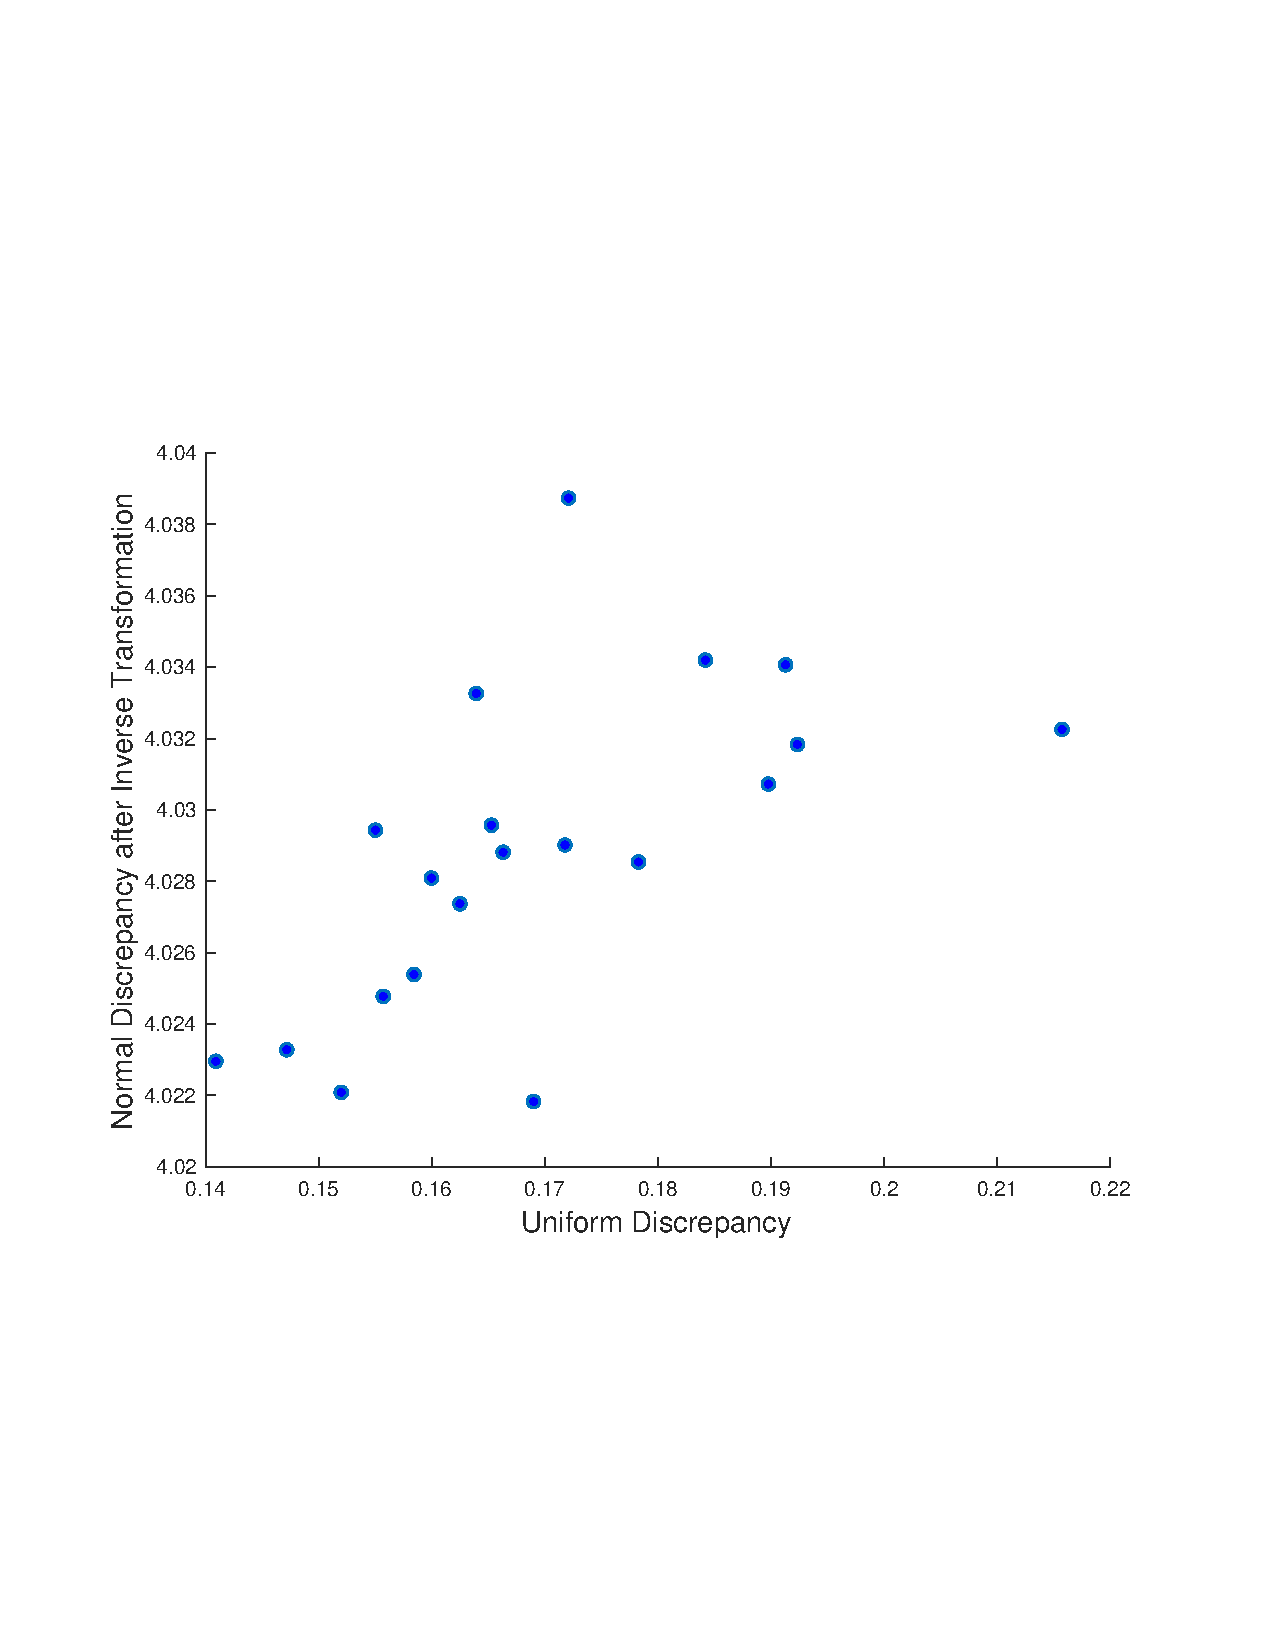
\includegraphics[width=8cm]{d5n50UniVsNormDisc2.pdf}}
\caption{Uniform Discrepancy Vs. Normal Discrepancy after Inverse Transformation}
\end{figure}

We further investigate the correlation between uniform discrepancy and the normal discrepancy after the inverse distribution transformation. For different variable dimension from $s=1$ to $s=10$, the sample correlation coefficients between the uniform discrepancies of 1000 uniform random samples of size 50 and the normal discrepancies of the corresponding normal random samples generated using inverse distribution transformation are calculated. From figure \ref{fig:UniVsNormDisc}, it can be seen that the phenomenon of inconsistency in discrepancy becomes more pronounced as the sample becomes more sparse.

\begin{figure}[htbp]
\label{fig:DimVsDisc}
\centering
{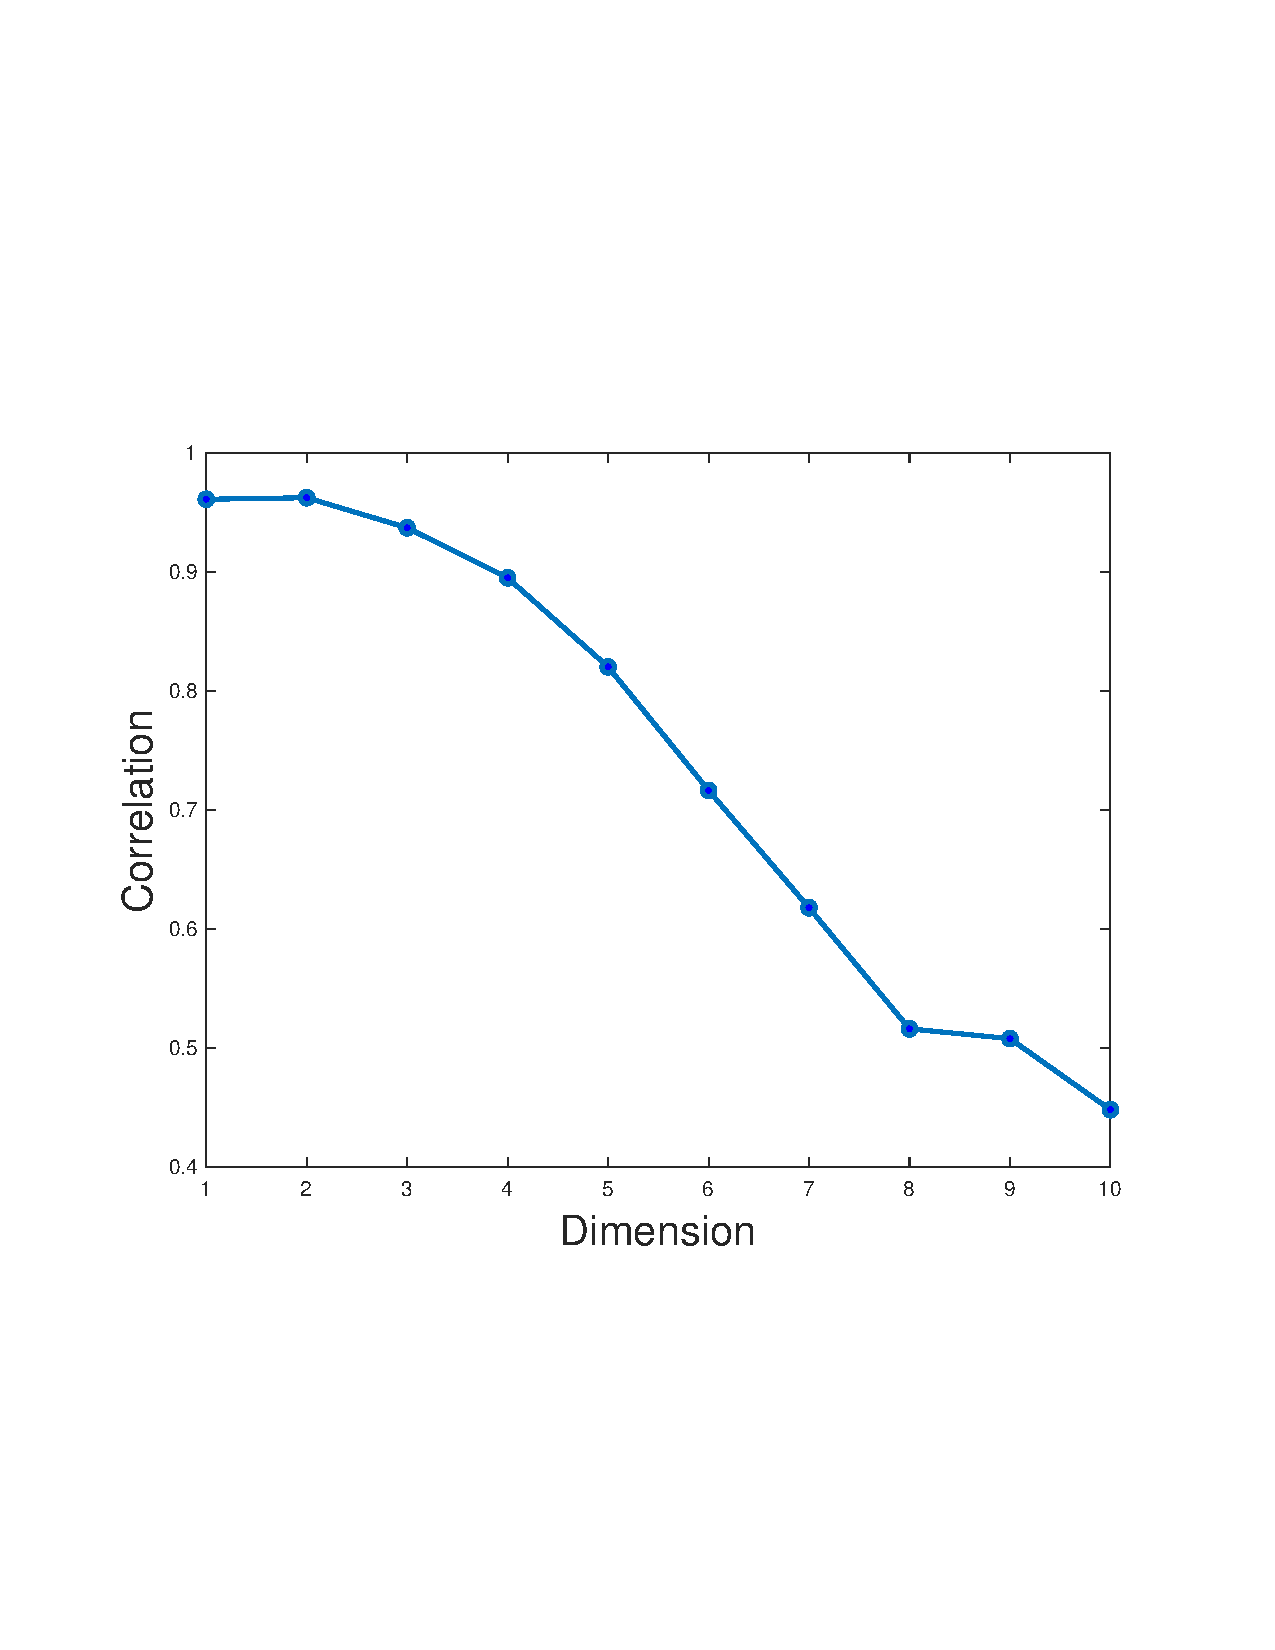
\includegraphics[width=8cm]{dimVsdisc.pdf}}
\caption{Correlation between Uniform Discrepancy and Normal Discrepancy with Different Variable Dimensions}
\end{figure}

\section{Improvement by the Coordinate-Exchange Algorithm}
The common practice to generate $d-$dim standard normal random numbers is inverse distribution transformation. However, as discussed in section \ref{sec:inconsistency}, a random sequence with low uniform discrepancy doesn't guarantee a low normal discrepancy sequence after inverse distribution transformation. We propose an efficient algorithm that assures low normal discrepancy of the generated $d$-dim standard normal random numbers.
\begin{algorithm}[ht]
\begin{algorithmic}[1]
\caption{Algorithm to generate a $d$-dim low normal discrepancy sequence}
\State Start with a $d$-dim low uniform discrepancy sequence, e.g., Sobol sequence 
\State 
\end{algorithmic}
\end{algorithm}
\section{Simulation}

\section{Conclusion}

\section*{Appendix}
Derivation of \eqref{eq:DisNormald=1} and \eqref{eq:DisNormald>1}. 
\begin{proof}
We first derive $[D(p)]^2$ for $d=1$ case. 
To compute the discrepancy, we first integrate the kernel once:
\begin{align*}
\MoveEqLeft{\int_{-\infty}^\infty K(x,t) \, \dif \Phi(x)}\\
=&\int_{-\infty}^{\infty} \left(1+\frac{1}{2}|x|+\frac{1}{2}|t|-\frac{1}{2}|x-t|\right)\phi(x) \, \dif x\\
=& 1+ \frac{1}{\sqrt{2\pi}} + \frac{1}{2}|t|-\frac{1}{2}\left[\int_{-\infty}^{t}(t-x)\phi(x) \, \dif x+\int_{t}^{\infty} (x-t)\phi(x) \, \dif x\right]\\
=& 1+ \frac{1}{\sqrt{2\pi}} + \frac{1}{2}|t| - t [\Phi(t)-1/2] - \phi(t) .
\end{align*}
Then we integrate again:
\begin{align*}
\MoveEqLeft{\int_{-\infty}^\infty \int_{-\infty}^\infty K(x,t) \, \dif \Phi(x) \dif \Phi(t)}\\
& =  \int_{-\infty}^{\infty} \left( 1+\frac{1}{\sqrt{2\pi}} + \frac{1}{2}|t| - t [\Phi(t)-1/2] + \phi(t)\right)\phi(t) \, \dif t\\
&= 1+ \sqrt{\frac{2}{\pi}} + \int_{-\infty}^{\infty} \{ - t \Phi(t)\phi(t)  +  [\phi(t)]^2 \} \, \dif t\\
&= 1+\sqrt{\frac{2}{\pi}}-\frac{1}{\sqrt{4\pi}}+\int_{-\infty}^{\infty}\frac{1}{2\pi}e^{-t^2}\dif t\\
&= 1+\sqrt{\frac{2}{\pi}}-\frac{1}{\sqrt{4\pi}}+\frac{\frac{1}{\sqrt{2}}}{\sqrt{2\pi}}\int_{-\infty}^{\infty}\frac{1}{\sqrt{2\pi}\left(\frac{1}{\sqrt{2}}\right)}e^{-\frac{t^2}{2\left(\frac{1}{\sqrt{2}}\right)^2}}\dif t\\
&=1+\sqrt{\frac{2}{\pi}}. 
\end{align*}
Notice that $\int_{-\infty}^{\infty} t\Phi(t)\phi(t)\dif t = \frac{1}{\sqrt{4\pi}}$ and 
\begin{eqnarray*}
&&\int_{\Omega}K(x,x_n)\dif \Phi(x)\\
&=& \int_{-\infty}^{\infty} \left(1+\frac{1}{2}|x|+\frac{1}{2}|x_n|-\frac{1}{2}|x-x_n|\right)\phi(x)\dif x\\
&=& 1+\frac{1}{2}\sqrt{\frac{2}{\pi}}+\frac{1}{2}|x_n|-\frac{1}{2}\left[\int_{-\infty}^{x_n}(x_n-x)\phi(x)\dif x+\int_{x_n}^{\infty} (x-x_n)\phi(x)\dif x\right]\\
&=& 1+\sqrt{\frac{1}{2\pi}}+\frac{1}{2}|x_n|-\frac{1}{2}\left[\int_{-\infty}^{x_n}(x_n-x)\phi(x)\dif x+\int_{x_n}^{\infty} (x-x_n)\phi(x)\dif x\right]\\
&=& 1+\sqrt{\frac{1}{2\pi}}+\frac{1}{2}|x_n|-\frac{1}{2}\left[2x_n\Phi(x_n)-x_n-2\int_{-\infty}^{x_n}x\phi(x)\dif x\right]\\
&=& 1+\sqrt{\frac{1}{2\pi}}+\max(x_n,0)-x_n\Phi(x_n)-\frac{ e^{-x_n^2/2}}{\sqrt{2\pi}}. 
\end{eqnarray*}
Thus, the discrepancy can be obtained as follows. 
\begin{eqnarray*}
&& [D(P)]^2\\
&= &1+\sqrt{\frac{2}{\pi}}-\frac{2}{N}\sum_{n=1}^N \left[1+\sqrt{\frac{1}{2\pi}}+\max(x_n,0)-x_n\Phi(x_n)-\frac{ e^{-x_n^2/2}}{\sqrt{2\pi}}\right]\\
&&+\frac{1}{N^2}\sum_{n,m=1}^N \left[1+\frac{1}{2}|x_n|+\frac{1}{2}|x_m|-\frac{1}{2}|x_n-x_m|\right]\\
&= &-\frac{2}{N}\sum_{n=1}^N \left[\max(x_n,0)-x_n\Phi(x_n)-\frac{ e^{-x_n^2/2}}{\sqrt{2\pi}}\right]+\frac{1}{N^2}\sum_{n,m=1}^N \left[\frac{1}{2}|x_n|+\frac{1}{2}|x_m|-\frac{1}{2}|x_n-x_m|\right]\\
&=& -\frac{2}{N}\sum_{n=1}^N \left[\max(x_n,0)-x_n\Phi(x_n)-\phi(x_n)\right]+\frac{1}{N}\sum_{n=1}^N|x_n|-\frac{1}{2N^2}\sum_{n,m=1}^N|x_n-x_m|.\\
\end{eqnarray*}
For the distribution $N({\bf 0}, {\bf I}_d)$, the joint pdf is $$\prod\limits_{j=1}^d\phi(x_j) = \prod\limits_{j=1}^d \frac{1}{\sqrt{2\pi}}e^{-x_j^2/2}.$$
Here the cdf function $\Phi$ used interchangeably for $N({\bf 0}, {\bf I}_d)$ and $N(0, 1)$, depending if the variable is a vector or scalar. Thus, 
\begin{align*}
\int_{\reals^d\times \reals^d} K(\vx,\vt)&\dif\Phi(\vx)\dif\Phi(\vt) = \left(1+\sqrt{\frac{2}{\pi}}\right)^d, \\
\int_{\reals^d}K(\vx,\vx_n)\dif\Phi(\vx) = \prod\limits_{j=1}^s&\left[ 1+\frac{1}{\sqrt{2\pi}}+\frac{1}{2}|x_j|-x_j[\Phi(x_j)-1/2]-\phi(x_j)\right].
\end{align*}
The discrepancy can be obtained
\begin{eqnarray*}
&&[D(P)]^2\\
&=& \left(1+\sqrt{\frac{2}{\pi}}\right)^d - \frac{2}{N}\sum\limits_{\vx\in P} \prod\limits_{j=1}^d\left[ 1+\frac{1}{\sqrt{2\pi}}+\frac{1}{2}|x_j|-x_j[\Phi(x_j)-1/2]-\phi(x_j)\right]\\
&&+\frac{1}{N^2}\sum_{\vx,\vt\in P}\prod_{j=1}^d \left[1+\frac{1}{2}|x_j|+\frac{1}{2}|t_j|-\frac{1}{2}|x_j-t_j|\right]. 
\end{eqnarray*}       
\end{proof}

\bibliographystyle{amsplain}
%\bibliography{FJH23,FJHown23}
\bibliography{Ref.bib}

\end{document}


